%===============================================================================
% $Id: ifacconf.tex 19 2011-10-27 09:32:13Z jpuente $  
% Template for IFAC meeting papers
% Copyright (c) 2007-2008 International Federation of Automatic Control
%===============================================================================
\documentclass{ifacconf}

\usepackage{graphicx}      % include this line if your document contains figures
\usepackage{natbib}        % required for bibliography
%===============================================================================
\begin{document}
\begin{frontmatter}

\title{Style for IFAC Conferences \& Symposia: Use Title Case for
  Paper Title\thanksref{footnoteinfo}} 
% Title, preferably not more than 10 words.

\thanks[footnoteinfo]{Sponsor and financial support acknowledgment
goes here. Paper titles should be written in uppercase and lowercase
letters, not all uppercase.}

\author[First]{First A. Author} 
\author[Second]{Second B. Author, Jr.} 
\author[Third]{Third C. Author}

\address[First]{National Institute of Standards and Technology, 
   Boulder, CO 80305 USA (e-mail: author@ boulder.nist.gov).}
\address[Second]{Colorado State University, 
   Fort Collins, CO 80523 USA (e-mail: author@lamar. colostate.edu)}
\address[Third]{Electrical Engineering Department, 
   Seoul National University, Seoul, Korea, (e-mail: author@snu.ac.kr)}

\begin{abstract}                % Abstract of not more than 250 words.
These instructions give you guidelines for preparing papers for IFAC
technical meetings. Please use this document as a template to prepare
your manuscript. For submission guidelines, follow instructions on
paper submission system as well as the event website.
\end{abstract}

\begin{keyword}
Five to ten keywords, preferably chosen from the IFAC keyword list.
\end{keyword}

\end{frontmatter}
%===============================================================================

\section{Introduction}
This document is a template for \LaTeXe. If you are reading a paper or
PDF version of this document, please download the electronic file
\texttt{ifacconf.tex}. You will also need the class file
\texttt{ifacconf.cls}. Both files are available on the IFAC web site.

Please stick to the format defined by the \texttt{ifacconf} class, and
do not change the margins or the general layout of the paper. It
is especially important that you do not put any running header/footer
or page number in the submitted paper.\footnote{
This is the default for the provided class file.}
Use \emph{italics} for emphasis; do not underline.

Page limits may vary from conference to conference. Please observe the 
page limits of the event for which your paper is intended.


\section{Procedure for Paper Submission}

Next we see a few subsections.

\subsection{Review Stage}

For submission guidelines, follow instructions on paper submission
system as well as the event website.

Note that conferences impose strict page limits, so it will be better
for you to prepare your initial submission in the camera ready layout
so that you will have a good estimate for the paper
length. Additionally, the effort required for final submission will be
minimal.

\subsection{Equations}

Some words might be appropriate describing equation~(\ref{eq:sample}), if 
we had but time and space enough. 

\begin{equation} \label{eq:sample}
{{\partial F}\over {\partial t}} = D{{\partial^2 F}\over {\partial x^2}}.
\end{equation}

See \cite{Abl:56}, \cite{AbTaRu:54}, \cite{Keo:58} and \cite{Pow:85}.

\subsubsection{Example.} This equation goes far beyond the
celebrated theorem ascribed to the great Pythagoras by his followers.

\begin{thm}   % use the thm environment for theorems
The square of the length of the hypotenuse of a right triangle equals
the sum of the squares of the lengths of the other two sides.
\end{thm}

\begin{pf}    % and the pf environment for proofs
The square of the length of the hypotenuse of a right triangle equals the sum of the squares 
of the lengths of the other two sides.
\end{pf}

%% There are a number of predefined theorem-like environments in
%% ifacconf.cls:
%%
%% \begin{thm} ... \end{thm}            % Theorem
%% \begin{lem} ... \end{lem}            % Lemma
%% \begin{claim} ... \end{claim}        % Claim
%% \begin{conj} ... \end{conj}          % Conjecture
%% \begin{cor} ... \end{cor}            % Corollary
%% \begin{fact} ... \end{fact}          % Fact
%% \begin{hypo} ... \end{hypo}          % Hypothesis
%% \begin{prop} ... \end{prop}          % Proposition
%% \begin{crit} ... \end{crit}          % Criterion

Of course LaTeX manages equations through built-in macros. You may
wish to use the \texttt{amstex} package for enhanced math
capabilities.

\subsection{Figures}

To insert figures, use the \texttt{graphicx} package. Although other
graphics packages can also be used, \texttt{graphicx} is simpler to
use. See  Fig.~\ref{fig:bifurcation} for an example.

\begin{figure}
\begin{center}
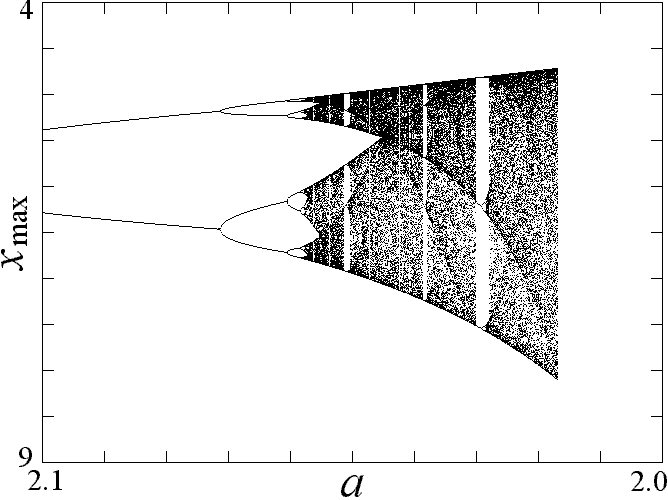
\includegraphics[width=8.4cm]{bifurcation}    % The printed column width is 8.4 cm.
\caption{Bifurcation: Plot of local maxima of $x$ with damping $a$ decreasing} 
\label{fig:bifurcation}
\end{center}
\end{figure}

Figures must be centered, and have a caption at the bottom. 

\subsection{Tables}
Tables must be centered and have a caption above them, numbered with
Arabic numerals. See table~\ref{tb:margins} for an example.

\begin{table}[hb]
\begin{center}
\caption{Margin settings}\label{tb:margins}
\begin{tabular}{cccc}
Page & Top & Bottom & Left/Right \\\hline
First & 3.5 & 2.5 & 1.5 \\
Rest & 2.5 & 2.5 & 1.5 \\ \hline
\end{tabular}
\end{center}
\end{table}

\subsection{Final Stage}

Authors are expected to mind the margins diligently.  Papers need to
be stamped with event data and paginated for inclusion in the
proceedings. If your manuscript bleeds into margins, you will be
required to resubmit and delay the proceedings preparation in the
process.

\subsubsection{Page margins.} See table~\ref{tb:margins} for the
page margins specification. All dimensions are in \emph{centimeters}.


\subsection{PDF Creation}

All fonts must be embedded/subsetted in the PDF file. Use one of the
following tools to produce a good quality PDF file:

\subsubsection{PDFLaTeX} is a special version of LaTeX by Han The
Thanh which produces PDF output directly using Type-1 fonts instead of
the standard \texttt{dvi} file. It accepts figures in JPEG, PNG, and PDF
formats, but not PostScript. Encapsulated PostScript figures can be
converted to PDF with the \texttt{epstopdf} tool or with Adobe Acrobat
Distiller.

\subsubsection{Generating PDF from PostScript} is the classical way of
producing PDF files from LaTeX. The steps are:

\begin{enumerate}
  \item Produce a \texttt{dvi} file by running \texttt{latex} twice.
  \item Produce a PostScript (\texttt{ps}) file with \texttt{dvips}.
  \item Produce a PDF file with \texttt{ps2pdf} or Adobe Acrobat
  Distiller.
\end{enumerate}

\subsection{Copyright Form}

IFAC will put in place an electronic copyright transfer system in due
course. Please \emph{do not} send copyright forms by mail or fax. More
information on this will be made available on IFAC website.


\section{Units}

Use SI as primary units. Other units may be used as secondary units
(in parentheses). This applies to papers in data storage. For example,
write ``$15\,\mathrm{Gb}/\mathrm{cm}^2$ ($100\,\mathrm{Gb}/\mathrm{in}^2$)''. 
An exception is when
English units are used as identifiers in trade, such as ``3.5 in
disk drive''. Avoid combining SI and other units, such as current in
amperes and magnetic field in oersteds. This often leads to confusion
because equations do not balance dimensionally. If you must use mixed
units, clearly state the units for each quantity in an equation.  The
SI unit for magnetic field strength $\mathbf{H}$ is $\mathrm{A}/\mathrm{m}$. However, if you wish to
use units of $\mathrm{T}$, either refer to magnetic flux density $\mathbf{B}$ or
magnetic field strength symbolized as $\mu_0\,\mathbf{H}$. Use the center dot to
separate compound units, e.g., ``$\mathrm{A} \cdot \mathrm{m}^2$''.

\section{Helpful Hints}

\subsection{Figures and Tables}

Figure axis labels are often a source of confusion. Use words rather
than symbols. As an example, write the quantity ``Magnetization'', or
``Magnetization M'', not just ``M''. Put units in parentheses. Do not
label axes only with units.  For example, write ``Magnetization
($\mathrm{A}/\mathrm{m}$)'' or ``Magnetization ($\mathrm{A} \mathrm{m}^{-1}$)'', not just
 ``$\mathrm{A}/\mathrm{m}$''. Do not
label axes with a ratio of quantities and units. For example, write
``Temperature ($\mathrm{K}$)'', not ``$\mbox{Temperature}/\mathrm{K}$''.

Multipliers can be especially confusing. Write ``Magnetization
($\mathrm{kA}/\mathrm{m}$)'' or ``Magnetization ($10^3 \mathrm{A}/\mathrm{m}$)''. Do not write
``Magnetization $(\mathrm{A}/\mathrm{m}) \times 1000$'' because the reader would not know
whether the axis label means $16000\,\mathrm{A}/\mathrm{m}$ or $0.016\,\mathrm{A}/\mathrm{m}$.

\subsection{References}

Use Harvard style references (see at the end of this document). With
\LaTeX, you can process an external bibliography database 
using \texttt{bibtex},\footnote{In this case you will also need the \texttt{ifacconf.bst}
file, which is part of the \texttt{ifaconf} package.}
or insert it directly into the reference section. Footnotes should be avoided as
far as possible.  Please note that the references at the end of this
document are in the preferred referencing style. Papers that have not
been published should be cited as ``unpublished''.  Capitalize only the
first word in a paper title, except for proper nouns and element
symbols.

\subsection{Abbreviations and Acronyms}

Define abbreviations and acronyms the first time they are used in the
text, even after they have already been defined in the
abstract. Abbreviations such as IFAC, SI, ac, and dc do not have to be
defined. Abbreviations that incorporate periods should not have
spaces: write ``C.N.R.S.'', not ``C. N. R. S.'' Do not use abbreviations
in the title unless they are unavoidable (for example, ``IFAC'' in the
title of this article).

\subsection{Equations}

Number equations consecutively with equation numbers in parentheses
flush with the right margin, as in (\ref{eq:sample}).  To make your equations more
compact, you may use the solidus ($/$), the $\exp$ function, or
appropriate exponents. Use parentheses to avoid ambiguities in
denominators. Punctuate equations when they are part of a sentence, as
in

\begin{equation} \label{eq:sample2}
\begin{array}{ll}
\int_0^{r_2} & F (r, \varphi ) dr d\varphi = [\sigma r_2 / (2 \mu_0 )] \\
& \cdot \int_0^{\inf} exp(-\lambda |z_j - z_i |) \lambda^{-1} J_1 (\lambda  r_2 ) J_0 (\lambda r_i ) d\lambda 
\end{array}
\end{equation}

Be sure that the symbols in your equation have been defined before the
equation appears or immediately following. Italicize symbols ($T$
might refer to temperature, but T is the unit tesla). Refer to
``(\ref{eq:sample})'', not ``Eq. (\ref{eq:sample})'' or ``equation
(\ref{eq:sample})'', except at the beginning of a sentence: ``Equation
(\ref{eq:sample}) is \ldots''.

\subsection{Other Recommendations}

Use one space after periods and colons. Hyphenate complex modifiers:
``zero-field-cooled magnetization''. Avoid dangling participles, such
as, ``Using (1), the potential was calculated'' (it is not clear who or
what used (1)). Write instead: ``The potential was calculated by using
(1)'', or ``Using (1), we calculated the potential''.

A parenthetical statement at the end of a sentence is punctuated
outside of the closing parenthesis (like this). (A parenthetical
sentence is punctuated within the parentheses.) Avoid contractions;
for example, write ``do not'' instead of ``don' t''. The serial comma
is preferred: ``A, B, and C'' instead of ``A, B and C''.


\section{Conclusion}

A conclusion section is not required. Although a conclusion may review
the main points of the paper, do not replicate the abstract as the
conclusion. A conclusion might elaborate on the importance of the work
or suggest applications and extensions.

\begin{ack}
Place acknowledgments here.
\end{ack}

\bibliography{ifacconf}             % bib file to produce the bibliography
                                                     % with bibtex (preferred)
                                                   
%\begin{thebibliography}{xx}  % you can also add the bibliography by hand

%\bibitem[Able(1956)]{Abl:56}
%B.C. Able.
%\newblock Nucleic acid content of microscope.
%\newblock \emph{Nature}, 135:\penalty0 7--9, 1956.

%\bibitem[Able et~al.(1954)Able, Tagg, and Rush]{AbTaRu:54}
%B.C. Able, R.A. Tagg, and M.~Rush.
%\newblock Enzyme-catalyzed cellular transanimations.
%\newblock In A.F. Round, editor, \emph{Advances in Enzymology}, volume~2, pages
%  125--247. Academic Press, New York, 3rd edition, 1954.

%\bibitem[Keohane(1958)]{Keo:58}
%R.~Keohane.
%\newblock \emph{Power and Interdependence: World Politics in Transitions}.
%\newblock Little, Brown \& Co., Boston, 1958.

%\bibitem[Powers(1985)]{Pow:85}
%T.~Powers.
%\newblock Is there a way out?
%\newblock \emph{Harpers}, pages 35--47, June 1985.

%\bibitem[Soukhanov(1992)]{Heritage:92}
%A.~H. Soukhanov, editor.
%\newblock \emph{{The American Heritage. Dictionary of the American Language}}.
%\newblock Houghton Mifflin Company, 1992.

%\end{thebibliography}

\appendix
\section{A summary of Latin grammar}    % Each appendix must have a short title.
\section{Some Latin vocabulary}              % Sections and subsections are supported  
                                                                         % in the appendices.
\end{document}
